\documentclass{article}
\oddsidemargin 0in \evensidemargin 0in \topmargin 0in
\columnsep 10pt \columnseprule 0pt 
\marginparwidth 90pt \marginparsep 11pt \marginparpush 5pt 
\headheight 0pt \headsep 0pt 
%\footheight 0pt \footskip 0pt 
\textheight 9.0in \textwidth 6.5in

\usepackage{graphicx}

\begin{document}

\begin{center}
{\large STATISTICS 201 - Written Homework Chapter 5}\\[6mm]
\end{center}

\noindent
This assignment is worth a total of 30 points.

\begin{enumerate}

\item (19 pts) The GRE is a test to measure undergraduate achievement and is used as an admissions criterion to graduate school. The GRE is designed in such a way that scores on the test can be modeled with a normal model. From July 2006 to June 2007 the mean GRE Verbal score was 457 with a standard deviation of 121. Use the z-table to answer the following questions. 

\begin{enumerate}
\item (3 pts) What proportion of all test takers will have a GRE Verbal score above 600 points?

The standardized value of 600 points is $z = \frac{600-457}{121} = 1.18182$ rounded to $z = 1.18$. 

The percentile from the normal table for $z = 1.18$ is $0.8810$. Since we want the proportion above 600 points, the answer is $1-0.8810 = 0.1190$.

\item (3 pts) What proportion of all test takers will have a GRE Verbal score below 375 points?

The standardized value of 375 points is $z = \frac{375-457}{121} = -0.677686$, rounded to $z = -0.68$. 

The percentile from the normal table for $z = -0.68$ is $0.2483$. Since we want the proportion below 375 points, the answer is $0.2483$. 

\item (5 pts) What proportion of all test takers will have a GRE Verbal score between 500 and 700 points?

The standardized value of 500 points is $z = \frac{500-457}{121} = 0.355372$, rounded to $z = 0.36$; the standardized value of 700 points is $z = \frac{700-457}{121} = 2.00826$, rounded to $z = 2.01$. 

The percentile from the normal table for $z = 0.36$ is 0.6406 and for $z = 2.01$ is 0.9778. Since we want the proportion between 500 and 700 points, the answer is $0.9778 - 0.6406 = 0.3372$.

\item (4 pts) What GRE Verbal score will 40\% of all test takers score below?

The score where 40\% of test takers are below is the same as the 40th percentile. From the normal table, the percentile closest to 0.40 is 0.4013 when $z = -0.25$, so we will use $z = -0.25$.

We are looking for the score that is 0.25 standard deviations below the mean, this value is $457 + (-0.25*121) = 426.75$.

\item (4 pts) What GRE verbal score will 10\% of all test takers score above?

The score where 10\% of test takers are above is the same score where 90\% are below. So we need to find the 90th percentile. From the normal table, the percentile 0.8997 when $z = 1.28$ is closest to 0.9, so we will use $z = 1.28$.  We are looking for the score that is 1.28 standard deviations above the mean, this value is $457 + (1.28*121) = 611.88$.

\end{enumerate}

\newpage

\item (11 pts) IIn a study to determine the nature of the relationship between heart rates and body temperature, body temperatures were collected from 130 individuals. The body temperatures, in degrees Fahrenheit, can be found in the  data file {\bf samplebodytemps.csv} in Blackboard.

Use the intRo software to determine if the distribution of body temperatures can be modeled with a normal model. Make sure to turn in the output from intRo with your assignment. In your answer, make sure to use information from the computer output that supports your conclusions. 

%\begin{tabular}{p{3in}p{2.5in}}
(5 pts) Computer output

\centerline{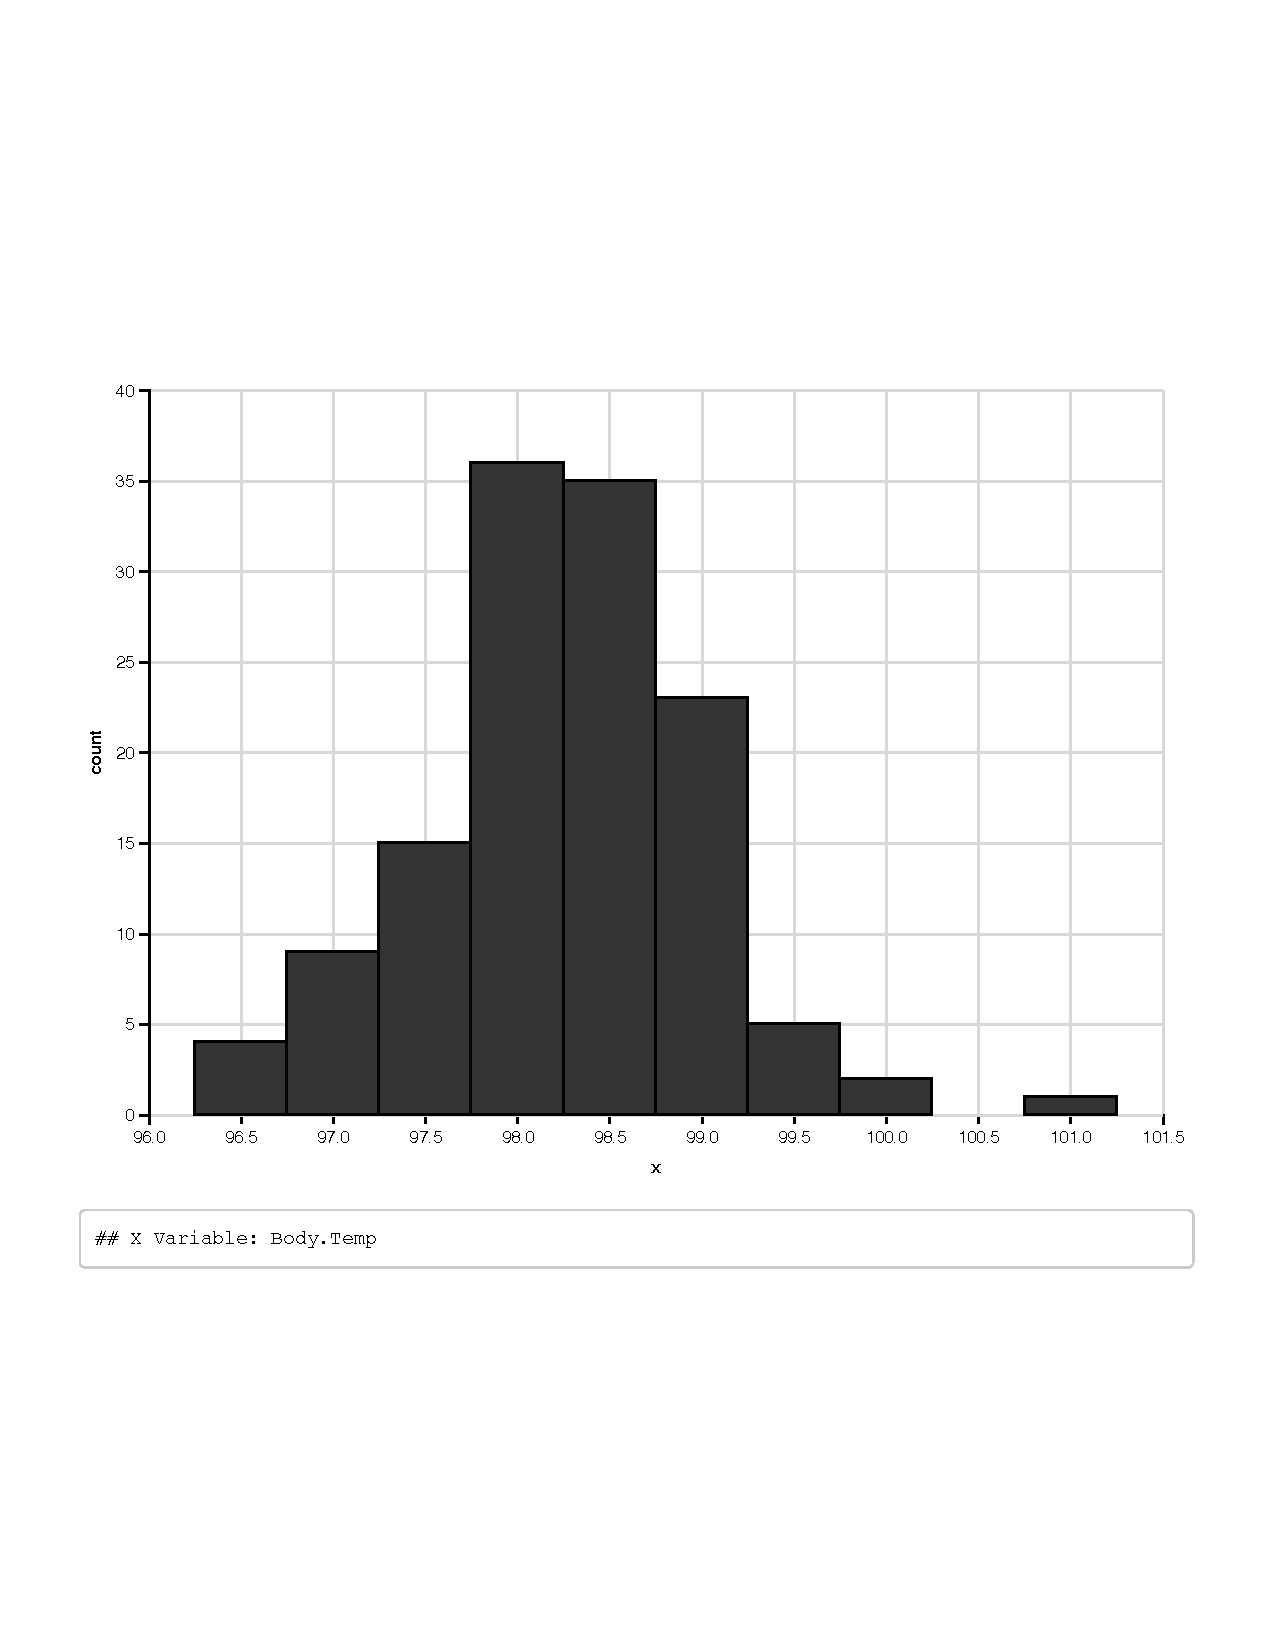
\includegraphics[width=3in]{hmwkch5-histogram.pdf}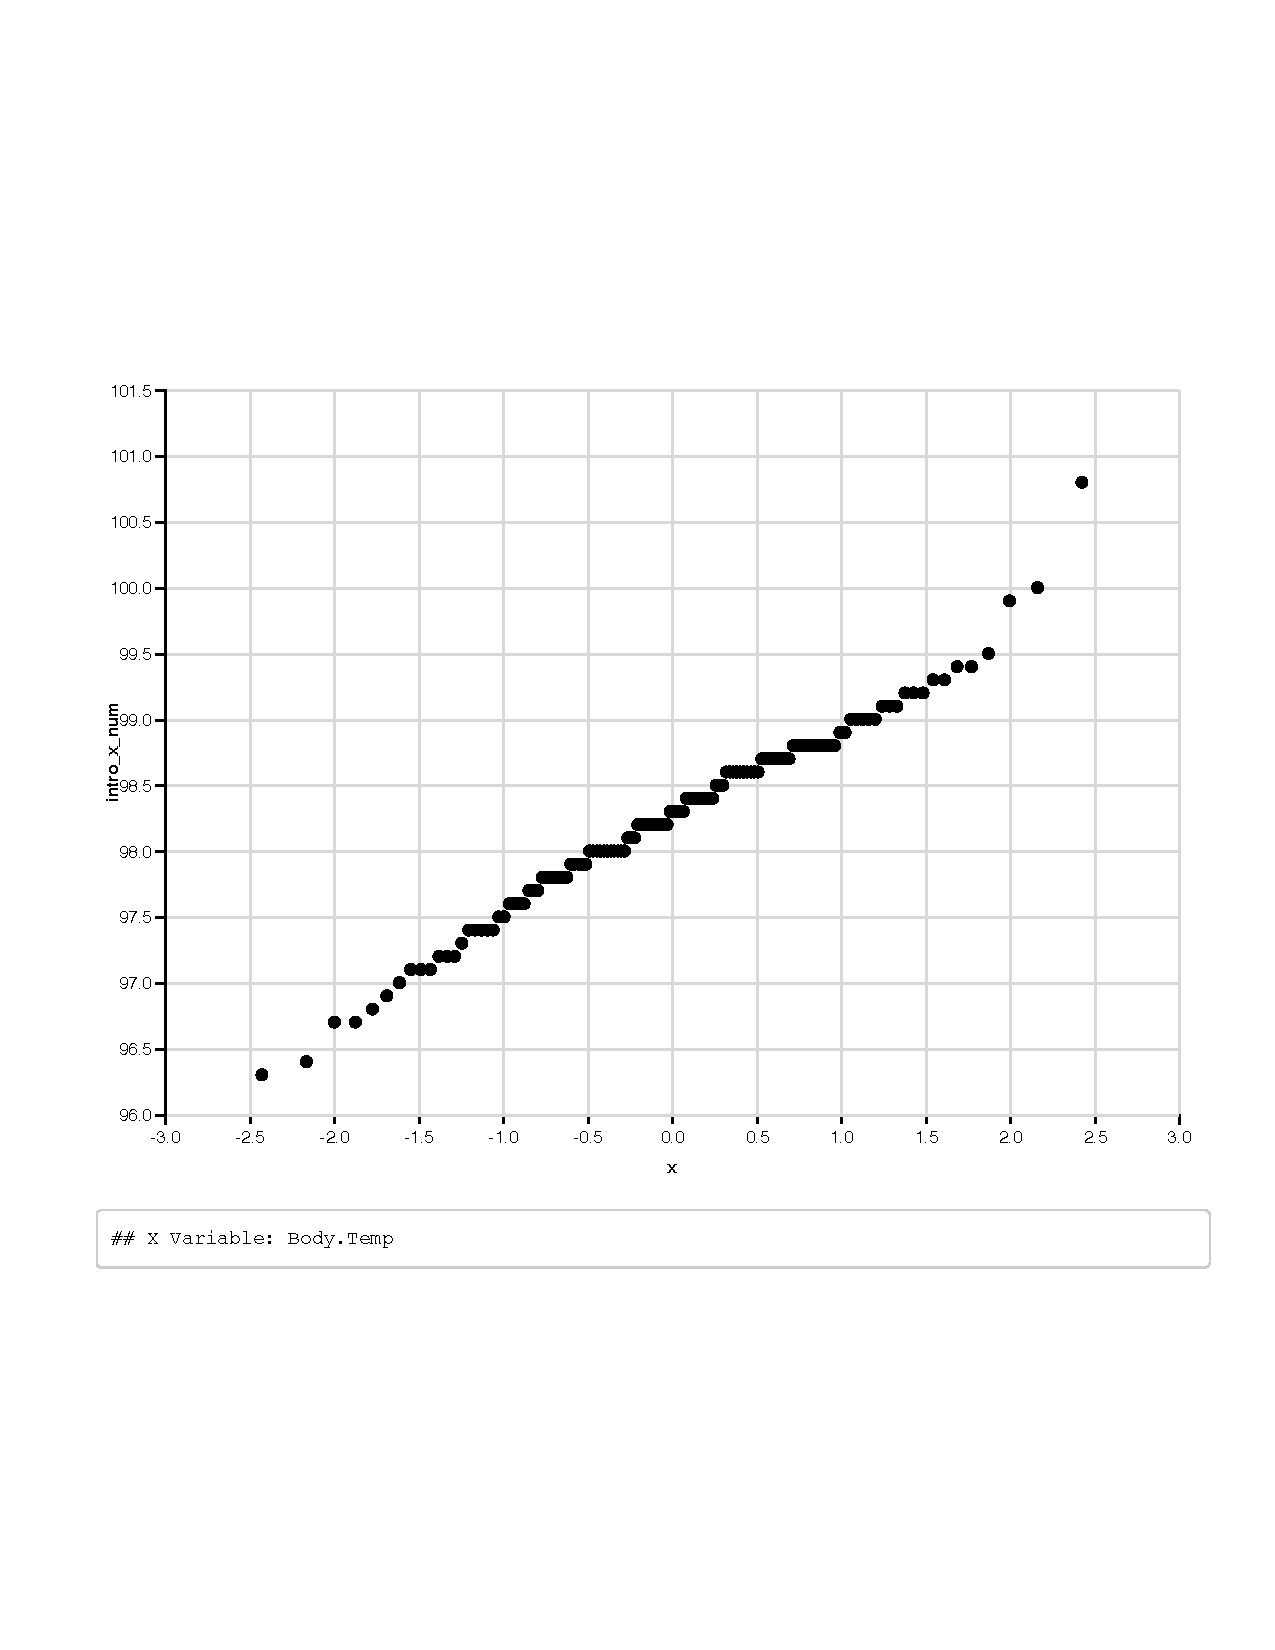
\includegraphics[width=3in]{hmwkch5-normprob.pdf}}

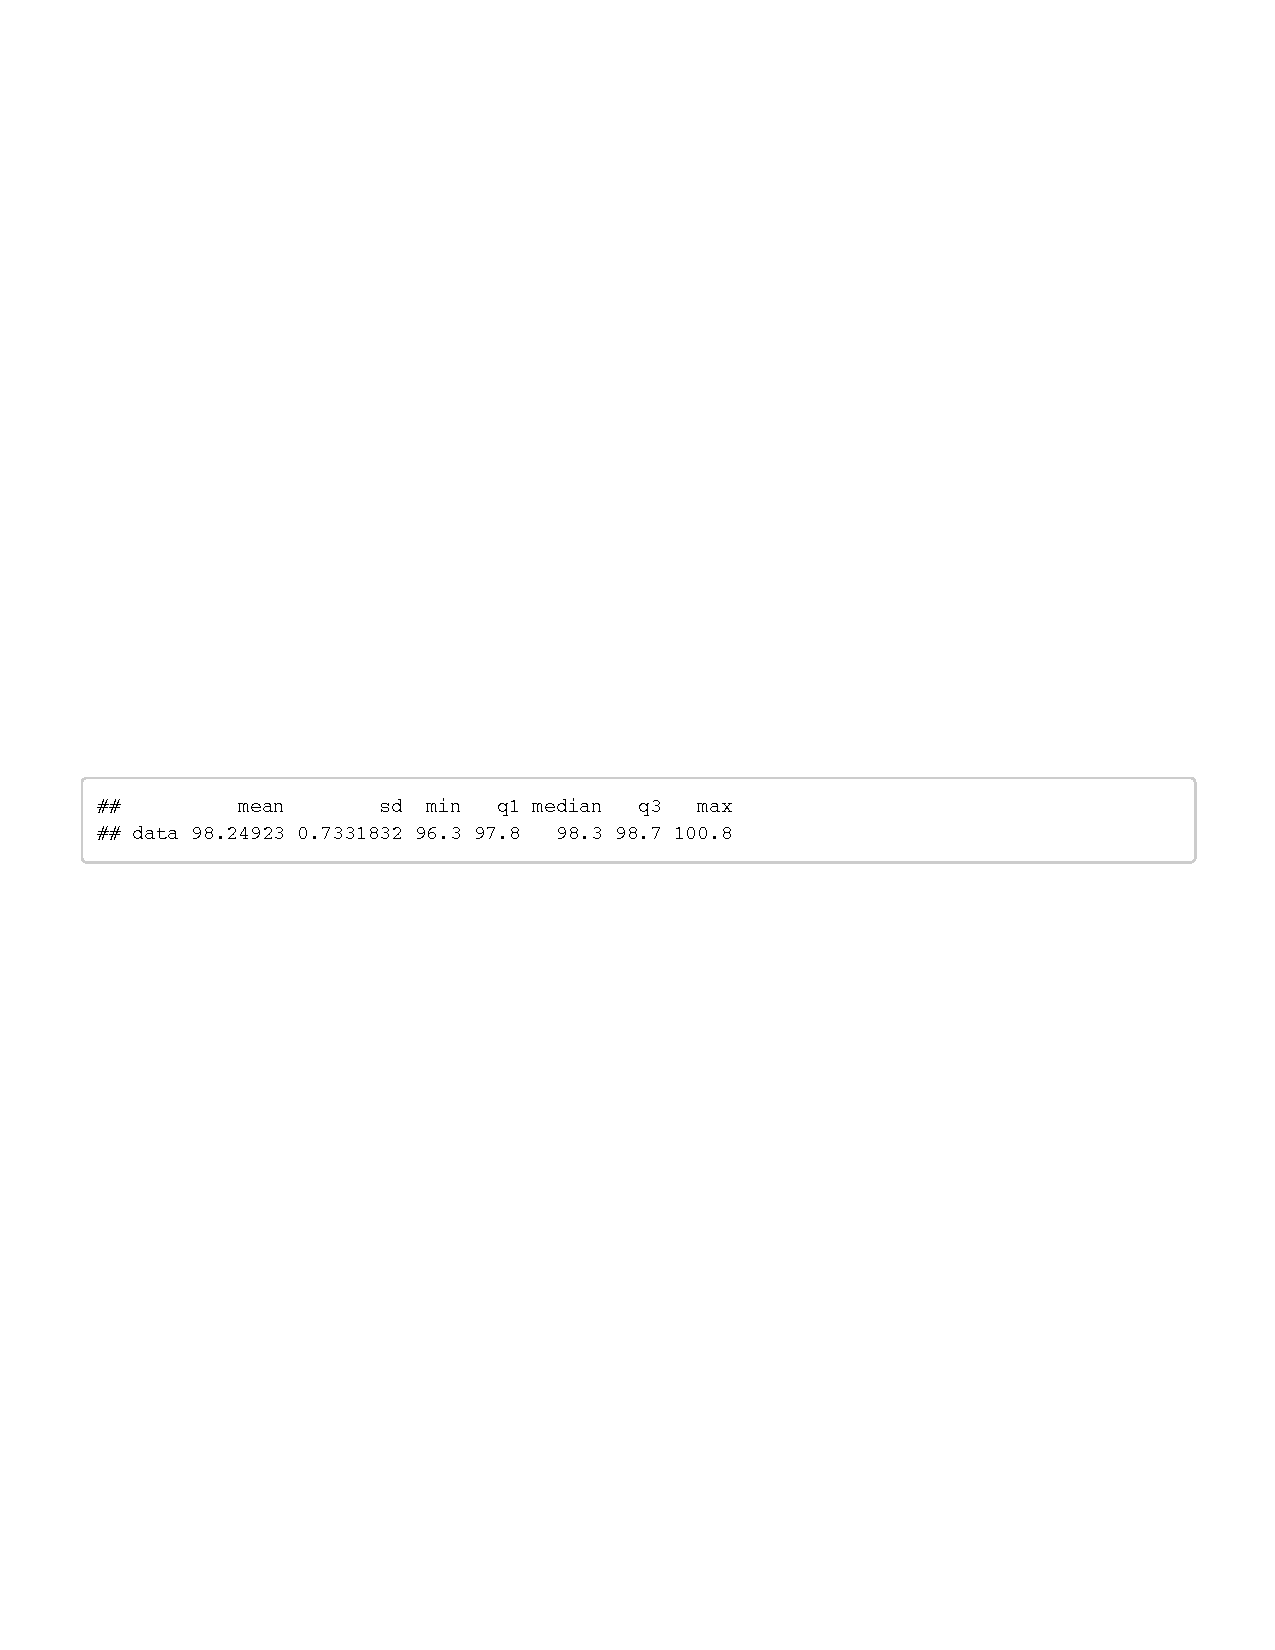
\includegraphics[width=6in]{hmwkch5-summary.pdf}

%&
%\vspace{0.5in}
(6 pts)  We see that the distribution of body temperatures is unimodal and symmetric, with a general bell-shape to the histogram.  The points in the normal quantile plot generally follow the straight line in the plot. Due to the shape of the histogram and the straight line pattern in the normal quantile plot.  We can also count the number of observations that fall within 1, 2, and 3 standard deviations to compare against the 68-95-99.7 rule. These are 90, 
123, 129 which corresponds to 69-95-99.2, extremely close to the ideal. 

It appears that the distribution of body temperatures in the sample can be modeled with the normal model.

%\end{tabular}

\end{enumerate}

\end{document}
